\chapter{Fundamentos da blockchain}
\label{chapter_fondamentos}


    O Blockchain é uma tecnologia nascente de 2009, usado por Nakamoto Satoshi \cite{Blockchain-Satochi},que está transformando o mundo da tecnologia e dos negócios por sua transparência, descentralização e propriedades de segurança. Desde então, ganhou muita atenção com a sua primeira aplicação de criptomoedas, como o Bitcoin.
    
    O conceito do blockchain, que é uma palavra em inglês e significa uma cadeia de blocos, foi apresentado por STUART HABER e AL em 1991 como um meio de marcar digitalmente documentos eletrônicos com data e horas para protegê-los contra adulteração \cite{anderson2020security}. A proposta inicial do Blockchain era resolver o problema da centralização, em que se precisava de terceiros confiáveis para processar uma transação digital \cite{9402747}.

    Assim que entra em ação a função do blockchain, que é definida nesse caso como uma cadeia de blocos digitais conectados e associados uns aos outros como um livro razão distribuído aberto que armazena informações sobre as operações que estão sendo feitas dentro dos blocos. A tecnologia Blockchain é aplicada em diferentes áreas e é diversificada em vários tipos, tais como:

        - Blockchains públicos: são aqueles que estão descentralizados e permitem a integração de qualquer pessoa à rede, assim conseguindo gerenciá-los.

        - Blockchains privados: são aqueles que só aceitam a integração de pessoas de uma única rede e gerenciá-las.

        - Blockchain de consórcio: são aqueles que estão entre os blockchains públicos e privados, em termos de permissões e gerenciamento. Eles permitem a integração de pessoas de várias organizações.

    O blockchain, como o próprio nome sugere, possui uma arquitetura especial que lhe confere as características mencionadas anteriormente. Ele é projetado para armazenar informações de forma eficiente e segura entre duas partes. No blockchain, as informações são organizadas em uma lista crescente, onde cada elemento dessa lista é chamado de bloco. É essa estrutura de blocos conectados que dá ao blockchain seu nome, "cadeia de blocos".\cite{9402747}

Além disso, é importante destacar que o blockchain é descentralizado, o que significa que não é controlado por uma única entidade ou autoridade central. Em vez disso, ele é mantido e verificado por uma rede de computadores distribuídos, chamados de nós, que trabalham em conjunto para validar e registrar as transações.\cite{tapscott2016technology}

Cada bloco do blockchain contém um conjunto de transações, que podem incluir informações como data, hora, valor e identificadores das partes envolvidas. Essas transações são verificadas e validadas pelos nós da rede, garantindo a integridade e a segurança do sistema.\cite{Blockchain-Satochi}

Além disso, o blockchain utiliza técnicas criptográficas avançadas para proteger as informações armazenadas. Cada bloco possui um código único, chamado de hash, que é gerado a partir dos dados do bloco e de seu bloco anterior(Figure \ref{Blockchain-arquiteture}). Isso cria uma ligação criptográfica entre os blocos, garantindo que qualquer alteração em um bloco anterior afetaria todos os blocos subsequentes, tornando a manipulação dos dados praticamente impossível.\cite{swan2015blockchain}

\begin{figure}[!htb]
\centering
\frame{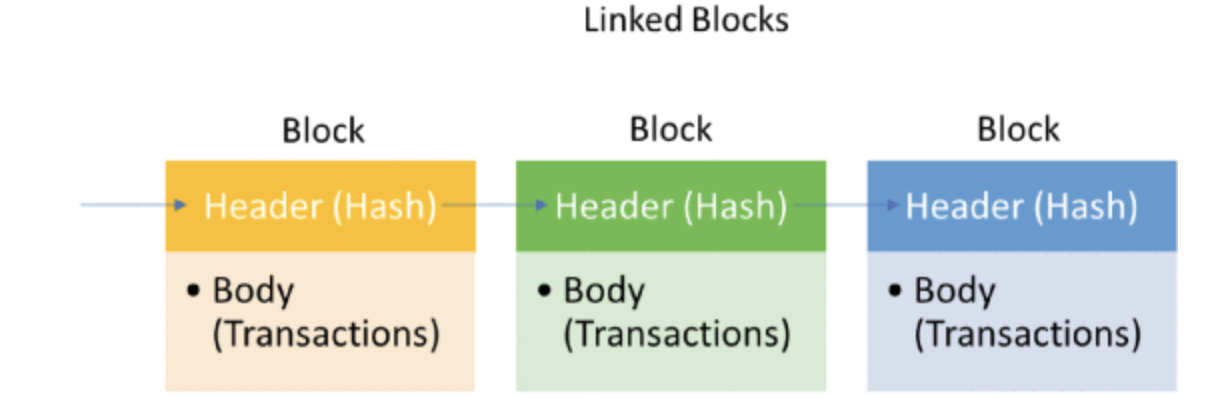
\includegraphics[width=15cm]{2-fundamentos-da-blockchain/figures/Blockchain-arch2.png}}
\caption{Blocks in the Blockchain architecture, \cite{9402747}, .}
\label{Blockchain-arquiteture}
\end{figure}

O blockchain, como mencionado anteriormente, é composto por blocos que estão interligados, permitindo o envio e recebimento de informações entre eles. Essa interconexão dos blocos forma uma rede caracterizada por nós. Existem duas categorias principais de nós: os nós completos e os nós leves. No entanto, é importante ressaltar que existem subnós que se diferenciam com base em suas funcionalidades específicas.

Os nós completos, também conhecidos como nós completos do blockchain, são responsáveis por manter uma cópia completa do registro de todas as transações ocorridas na rede blockchain. Esses nós possuem um alto nível de participação na rede e desempenham um papel crucial na validação e consenso das transações. Eles têm a capacidade de verificar todas as transações e armazenar uma cópia completa do blockchain, o que requer um grande poder de processamento e espaço de armazenamento.\cite{9402747}

Por outro lado, os nós leves, também chamados de nós-cliente, têm uma funcionalidade mais limitada em comparação aos nós completos. Esses nós não armazenam uma cópia completa do blockchain, mas apenas informações relevantes para suas operações específicas. Eles dependem dos nós completos para acessar o blockchain e verificar as transações. Os nós leves são mais leves em termos de requisitos de recursos, tornando-os adequados para dispositivos com capacidade de processamento e armazenamento limitados, como smartphones e dispositivos de IoT (Internet das Coisas).

Dentro dessas categorias, existem subnós com funcionalidades especializadas, como os nós mineradores. Os nós mineradores são responsáveis por adicionar novos blocos à cadeia, utilizando poder computacional para resolver problemas matemáticos complexos, conhecidos como prova de trabalho (proof-of-work). Eles desempenham um papel crucial na manutenção da segurança e integridade do blockchain, garantindo que apenas transações válidas sejam adicionadas aos blocos.

Essa estrutura de nós no blockchain permite a descentralização e a distribuição das informações, aumentando a segurança e a transparência do sistema. Cada nó na rede possui uma cópia do blockchain e participa da validação e consenso das transações.(Figure \ref{Blockchain-Nodes}).


\begin{figure}[!htb]
\centering
\frame{\includegraphics[width=15cm]{2-fundamentos-da-blockchain/figures/Capture d’écran 2023-12-03 à 23.07.25.png}}
\caption{Estrutua do Blockchain.}
\label{Blockchain-Nodes}
\end{figure}

